\chapter{Abbreviations}
{
    \renewcommand*{\arraystretch}{1.1}
    \begin{table}[htbp]
        \centering
        \begin{tabular}{rp{0.6\textwidth}} 
            \toprule
            Abbreviation & Meaning\\
            \midrule 
            (D/F)CNN & (Deep-/Fully-) Convolutional Neural Network; a (deep) neural network that (only) includes convolutional layers in its main path\\
            SAW & Surface Acoustic Wave\\
            IDT & Interdigital Transducer\\
            lr & learning rate\\
            lrsp & learning rate scheduler patience\\
            lrsf & \linespread{1.0}\selectfont learning rate scheduler factor; the number the learning rate is multiplied by in case the scheduler detects stagnant progress\\
            bs, bsize & batch size\\
            lbls & labeled samples \\
            MT & Mean Teacher \\
            EMA & Exponential Moving Average \\
            sf & \linespread{1.0}\selectfont split factor; the number the height and width of the images and masks in the dataset are divided by for splitting them into smaller samples\\
            \bottomrule
        \end{tabular}
        \vspace{0.1cm}
        \caption{A list of abbreviations used in this thesis. The table explains the full meaning of each abbreviation as well as a short description if it is not obvious.}
        \label{tab:abbreviations}
    \end{table}
}

\chapter{Example Images}
~
\vfill
\begin{figure}[htbp]\ContinuedFloat*
    \centering
    \begin{subfigure}{\textwidth}
        \centering
            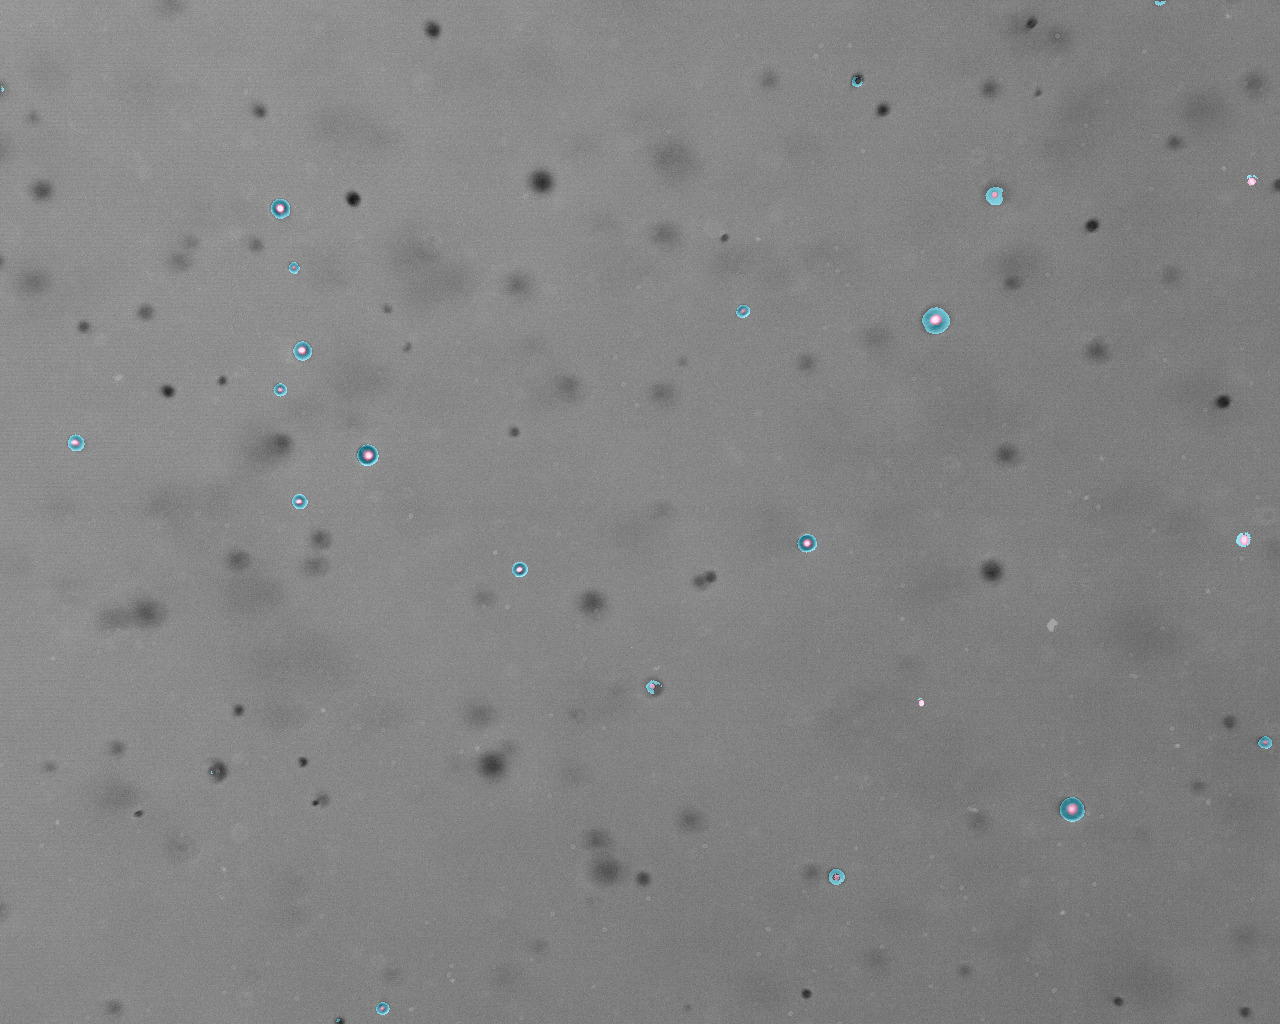
\includegraphics[width=\textwidth]{images/samples/36dbm_C001H001S0001000046_leftImg8bit_overlay.jpeg}
        \caption{Mask overlay for example image 1.}
    \end{subfigure}
\end{figure}
\vfill
~
\vfill
\begin{figure}[htbp]\ContinuedFloat
    \begin{subfigure}{\textwidth}
        \centering
            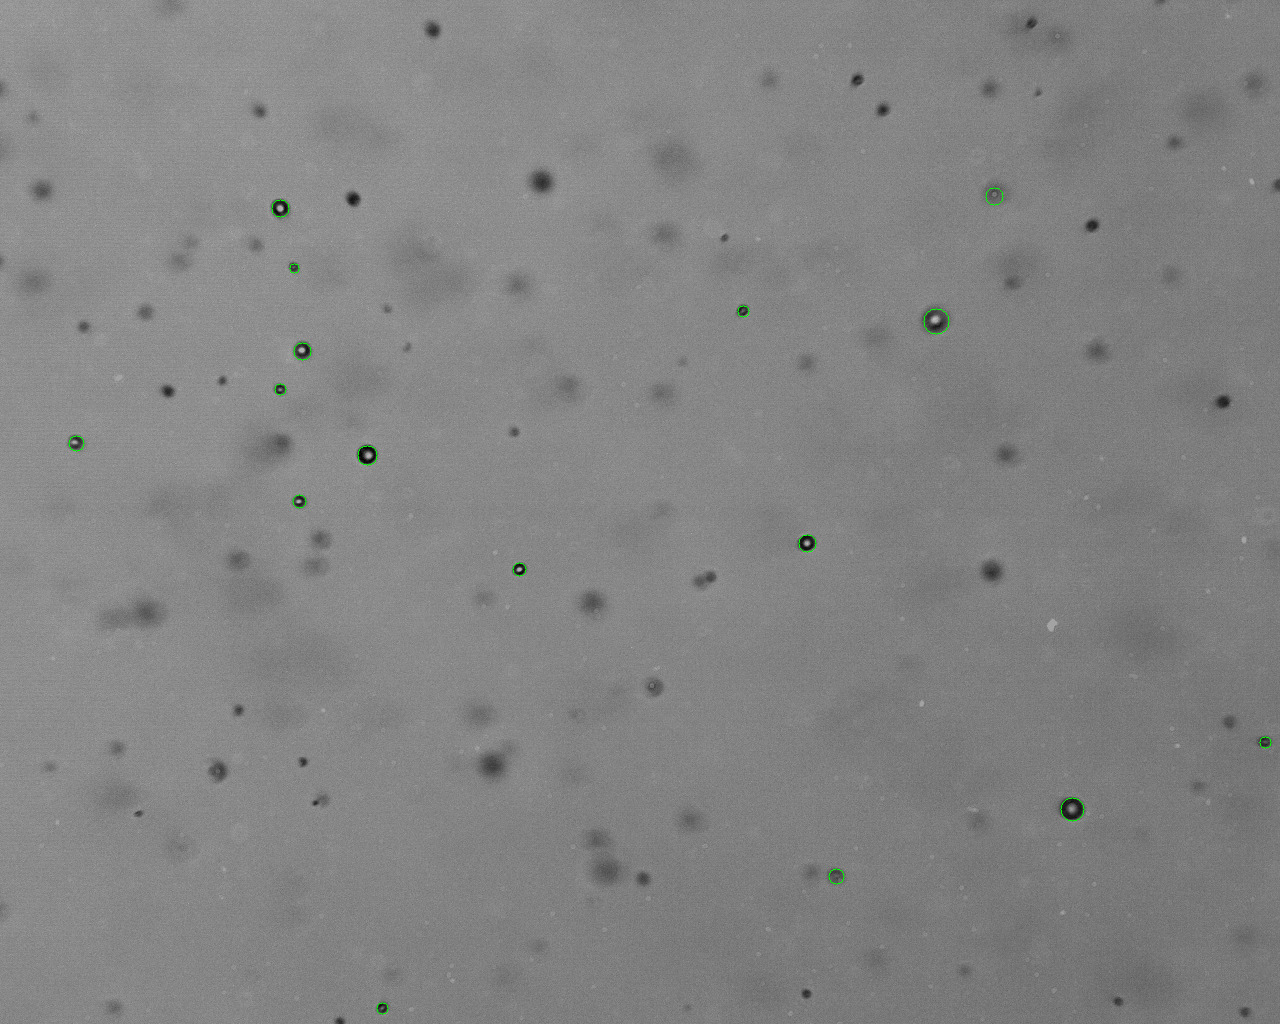
\includegraphics[width=\textwidth]{images/samples/36dbm_C001H001S0001000046_leftImg8bit_detected.jpeg}
        \caption{Detected droplets for example image 1.}
    \end{subfigure}
\end{figure}
~
\vfill
~
\begin{figure}[htbp]\ContinuedFloat
    \centering
    \begin{subfigure}{\textwidth}
        \centering
            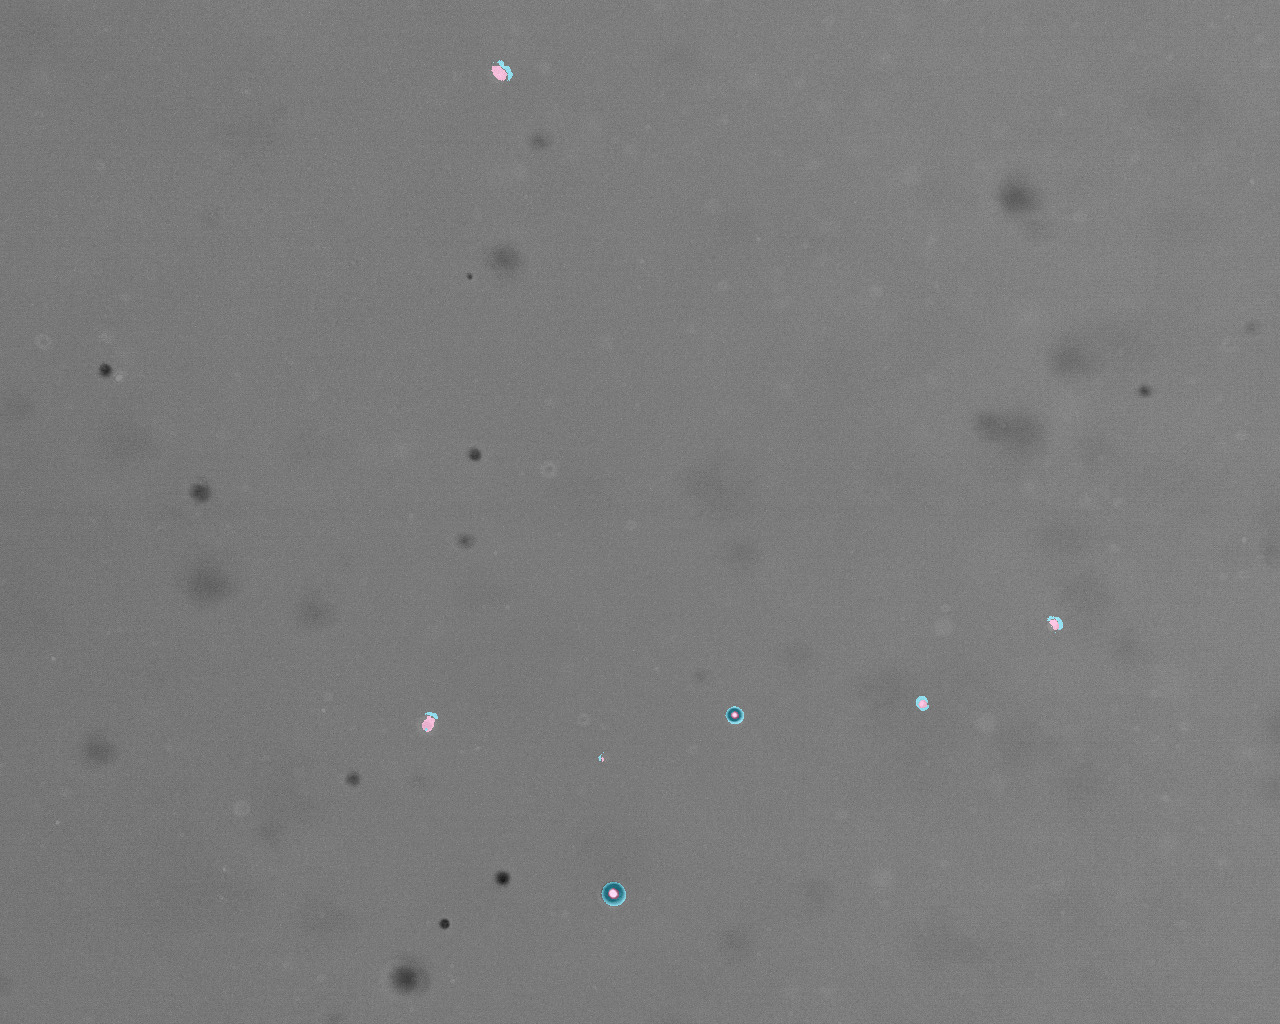
\includegraphics[width=\textwidth]{images/samples/36dbm_C001H001S0001000205_leftImg8bit_overlay.jpeg}
        \caption{Mask overlay for example image 2.}
    \end{subfigure}
\end{figure}
\vfill
~
\vfill
\begin{figure}[htbp]\ContinuedFloat
    \begin{subfigure}{\textwidth}
        \centering
            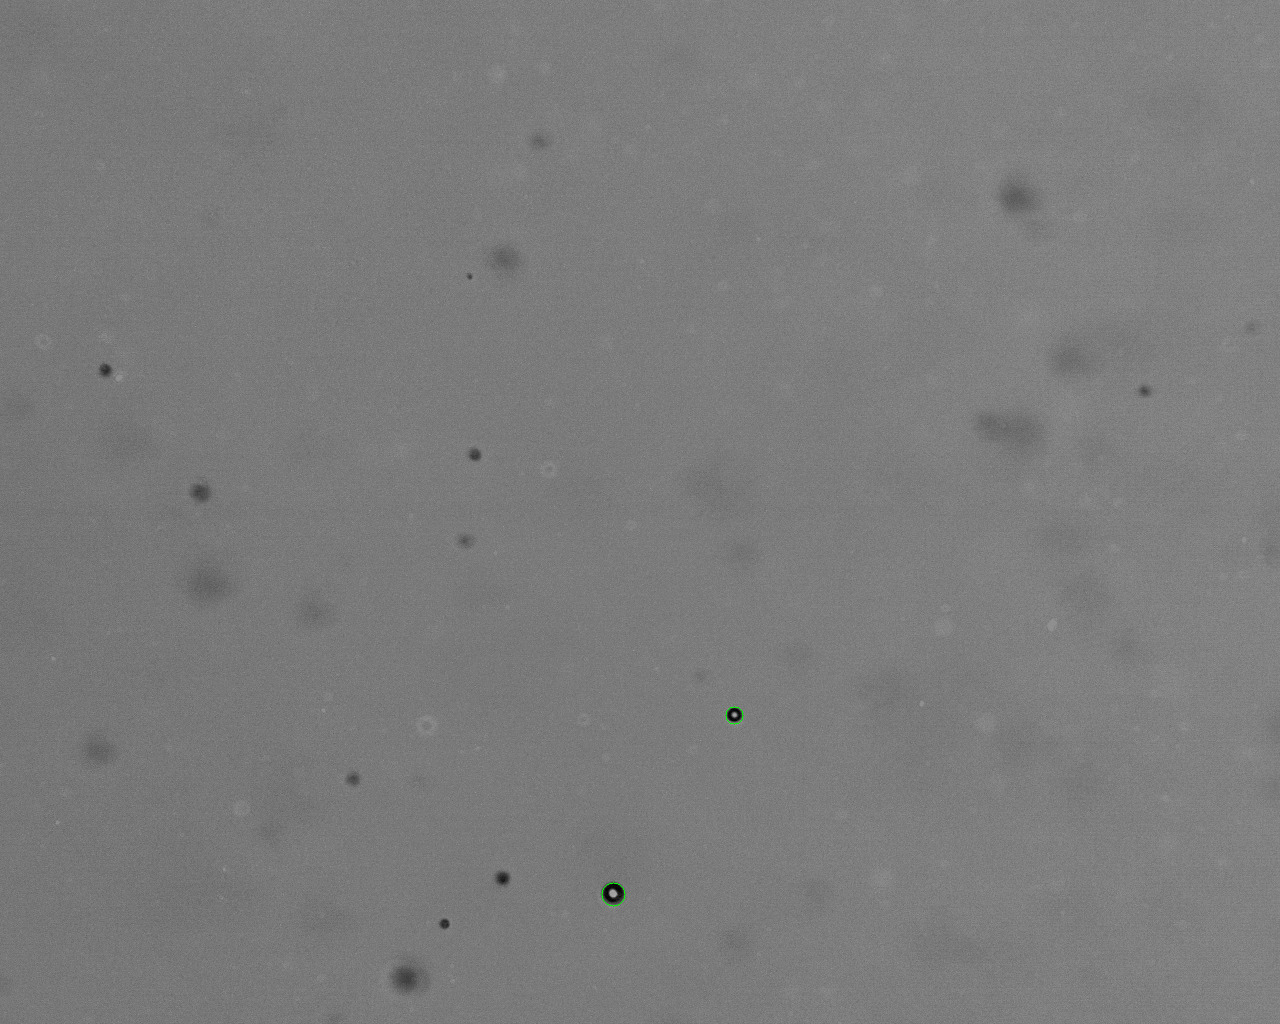
\includegraphics[width=\textwidth]{images/samples/36dbm_C001H001S0001000205_leftImg8bit_detected.jpeg}
        \caption{Detected droplets for example image 2.}
    \end{subfigure}
\end{figure}
~
\vfill
~
\begin{figure}[htbp]\ContinuedFloat
    \centering
    \begin{subfigure}{\textwidth}
        \centering
            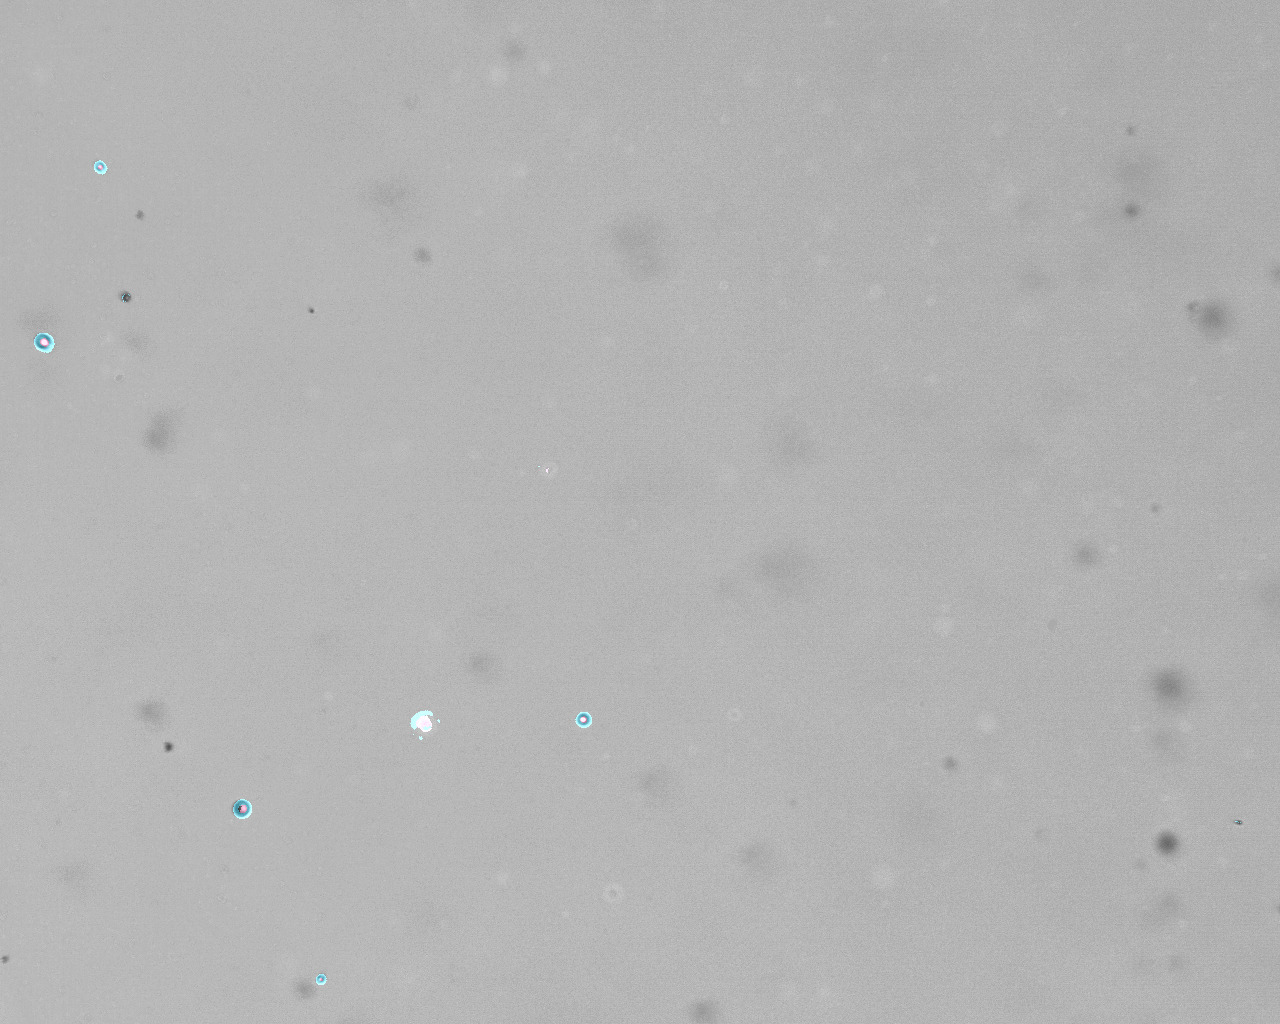
\includegraphics[width=\textwidth]{images/samples/36dbm_C001H001S0001000206_leftImg8bit_overlay.jpeg}
        \caption{Mask overlay for example image 3.}
    \end{subfigure}
\end{figure}
\vfill
~
\vfill
\begin{figure}[htbp]\ContinuedFloat
    \begin{subfigure}{\textwidth}
        \centering
            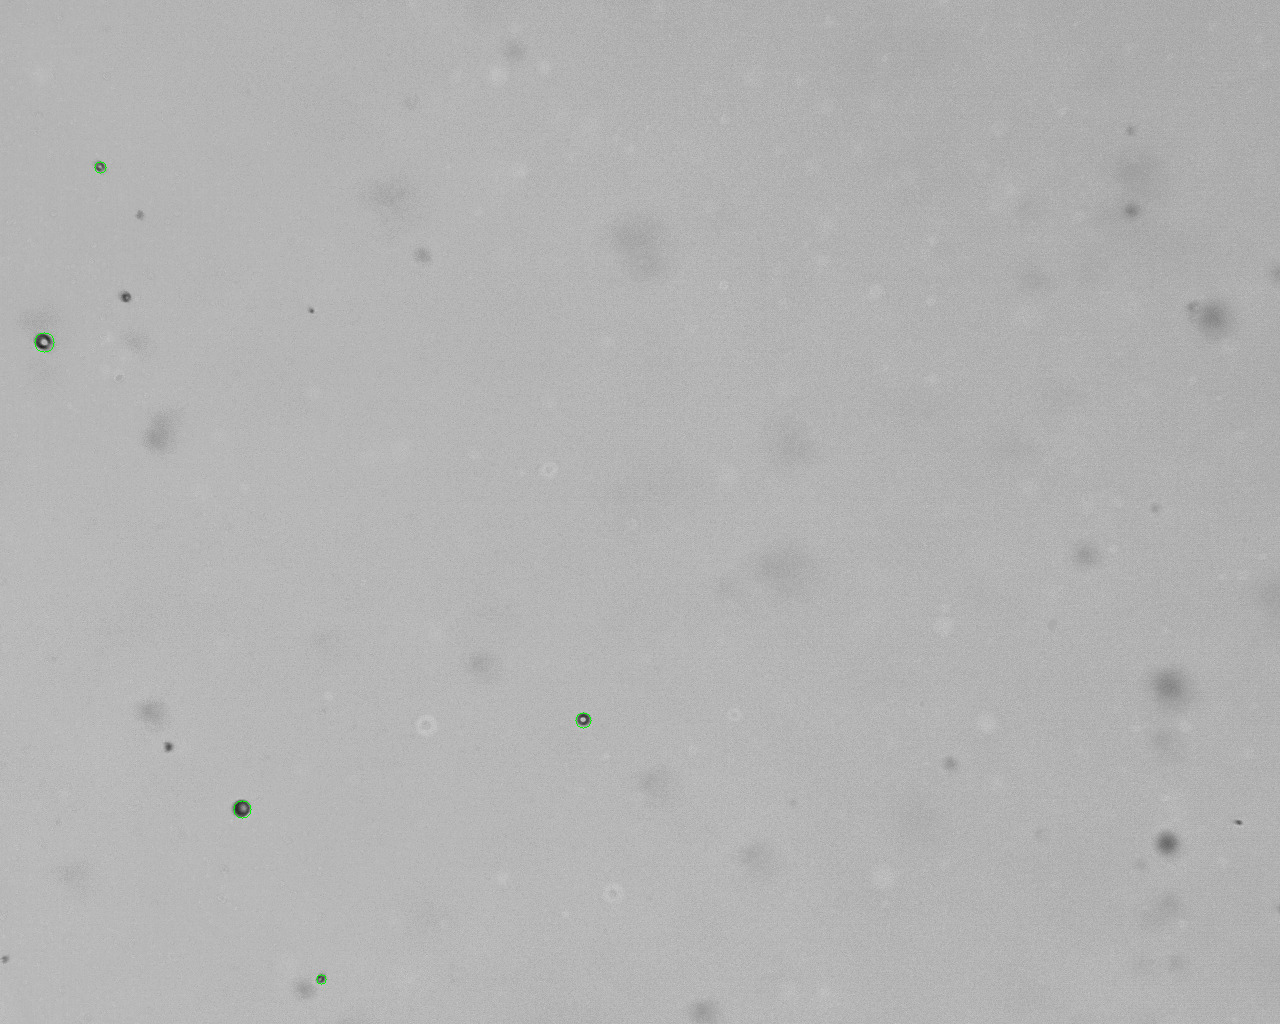
\includegraphics[width=\textwidth]{images/samples/36dbm_C001H001S0001000206_leftImg8bit_detected.jpeg}
        \caption{Detected droplets for example image 3.}
    \end{subfigure}
    \caption{Examples for some of the results from applying the measurement technique developed in the thesis. The images show the overlayed segmentation masks with blue for the droplets border labels and pink for the droplet center labels, as well as the droplets detected after filtering as green circles.}
    \label{fig:example_images}
\end{figure}
